\section{ASCbase::model\_\-hbond\_\-surf\_\-t Class Reference}
\label{classASCbase_1_1model__hbond__surf__t}\index{ASCbase::model_hbond_surf_t@{ASCbase::model\_\-hbond\_\-surf\_\-t}}
{\tt \#include $<$Model\-Hbond\-Surfaces.H$>$}

Inheritance diagram for ASCbase::model\_\-hbond\_\-surf\_\-t::\begin{figure}[H]
\begin{center}
\leavevmode
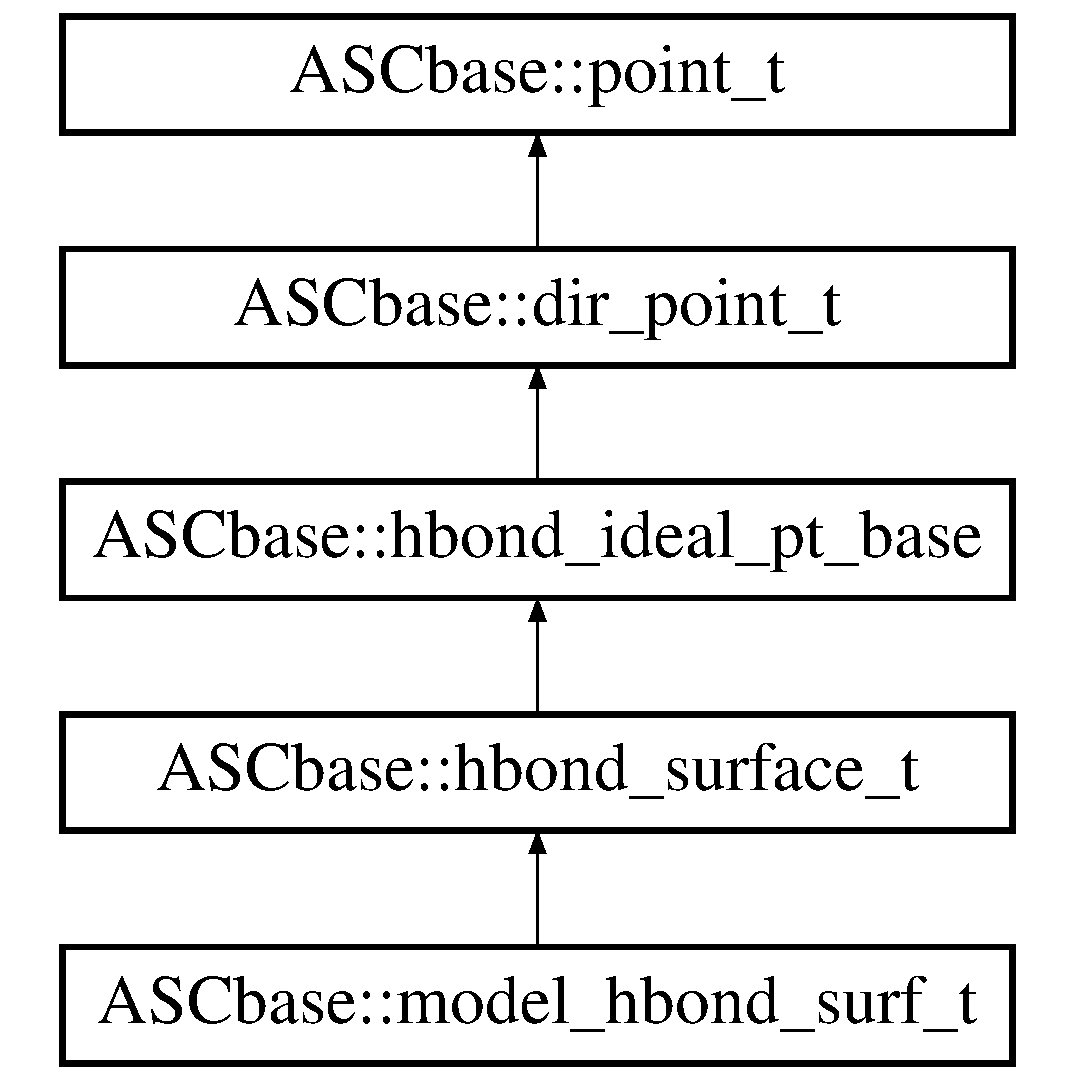
\includegraphics[height=5cm]{classASCbase_1_1model__hbond__surf__t}
\end{center}
\end{figure}
\subsection*{Public Member Functions}
\begin{CompactItemize}
\item 
\textbf{model\_\-hbond\_\-surf\_\-t} (const std::string \&data\_\-line, \bf{PDBBase} \&prot\_\-atoms, const uint level=2)\label{classASCbase_1_1model__hbond__surf__t_cb646a3dbc03f4990450144a918753a8}

\item 
\textbf{model\_\-hbond\_\-surf\_\-t} (const \bf{model\_\-hbond\_\-surf\_\-t} \&src)\label{classASCbase_1_1model__hbond__surf__t_c6978b9984df3bdd11e5b492600468c2}

\item 
\bf{model\_\-hbond\_\-surf\_\-t} \& \textbf{operator=} (const \bf{model\_\-hbond\_\-surf\_\-t} \&src)\label{classASCbase_1_1model__hbond__surf__t_01930d6fccfbfb3c509b686060699606}

\item 
void \textbf{transform} (const my\_\-float\_\-t $\ast$R, const my\_\-float\_\-t $\ast$T)\label{classASCbase_1_1model__hbond__surf__t_65d5a73c0ffcbada1c8496c81a43929a}

\item 
void \textbf{inverse\_\-transform} (const my\_\-float\_\-t $\ast$R, const my\_\-float\_\-t $\ast$T)\label{classASCbase_1_1model__hbond__surf__t_b0ebe991b54fb1b3247a4a716a0673d4}

\item 
void \textbf{revert} ()\label{classASCbase_1_1model__hbond__surf__t_da904de58db5258030d9144908f915c6}

\item 
void \bf{compute\_\-best\_\-terms} (std::vector$<$ \bf{hbond\_\-surface\_\-t} $>$::iterator surfs\_\-begin, std::vector$<$ \bf{hbond\_\-surface\_\-t} $>$::iterator surfs\_\-end, my\_\-float\_\-t $\ast$AA\_\-DD\_\-terms, my\_\-float\_\-t $\ast$doneptor\_\-terms, my\_\-float\_\-t $\ast$surface\_\-area, const my\_\-float\_\-t dist\_\-tol=1.0) const 
\begin{CompactList}\small\item\em Compute the best terms for each vertex in the model surface. \item\end{CompactList}\item 
const uint \textbf{num\_\-terms} () const \label{classASCbase_1_1model__hbond__surf__t_d29013b948a3de1594b72640d8f54aa0}

\item 
const uint \textbf{num\_\-verts} () const \label{classASCbase_1_1model__hbond__surf__t_7a0344de6eb971227cf37c96b0b11606}

\item 
const geometry::vertex\_\-vci \bf{verts\_\-begin} () const \label{classASCbase_1_1model__hbond__surf__t_fad5a5374d17a84192f1f8fc74ea8876}

\begin{CompactList}\small\item\em Get a constant iterator to the first vertex in the vector. \item\end{CompactList}\item 
const geometry::vertex\_\-vci \bf{verts\_\-end} () const \label{classASCbase_1_1model__hbond__surf__t_50ec409886843895685f8549707ba15e}

\begin{CompactList}\small\item\em Get a constant iterator to the end of the vertex vector. \item\end{CompactList}\item 
const my\_\-float\_\-t $\ast$ \bf{closest\_\-pts\_\-begin} () const \label{classASCbase_1_1model__hbond__surf__t_d97fb2ca02976980a4c1e78b46b0df63}

\begin{CompactList}\small\item\em Get a constant pointer to the first point in the closest points array. \item\end{CompactList}\item 
const my\_\-float\_\-t $\ast$ \bf{closest\_\-pts\_\-end} () const \label{classASCbase_1_1model__hbond__surf__t_dd599b65e329040ffdaea701a3acbaeb}

\begin{CompactList}\small\item\em Get a constant pointer to the end of the closest points array. \item\end{CompactList}\item 
const my\_\-float\_\-t $\ast$ \bf{closest\_\-pts\_\-dists\_\-begin} () const \label{classASCbase_1_1model__hbond__surf__t_05e5c2efb6bd80474c20a983c10324ff}

\begin{CompactList}\small\item\em Get a constant pointer to the first distance in the distances array. \item\end{CompactList}\item 
const my\_\-float\_\-t $\ast$ \bf{closest\_\-pts\_\-dists\_\-end} () const \label{classASCbase_1_1model__hbond__surf__t_a0183e08be99f865caa5c59f0441529f}

\begin{CompactList}\small\item\em Get a constant pointer to the end of the distances array. \item\end{CompactList}\item 
void \textbf{write} (std::ostream \&out, const interaction\-Type point\_\-type, const char delim='$|$') const \label{classASCbase_1_1model__hbond__surf__t_2c3b46d219e290bd39bf60cdc9210fcc}

\item 
void \textbf{write\_\-msms\_\-headers} (std::ostream \&vert\_\-out, std::ostream \&face\_\-out) const \label{classASCbase_1_1model__hbond__surf__t_ac5245563487a78bec4f41d973dae1ef}

\item 
void \textbf{write\_\-msms\_\-cap} (std::ostream \&vert\_\-out, std::ostream \&face\_\-out) const \label{classASCbase_1_1model__hbond__surf__t_b7a5a82b5ba33c13c2f1fde5e2c68e93}

\end{CompactItemize}
\subsection*{Private Member Functions}
\begin{CompactItemize}
\item 
bool \textbf{adjust\_\-terms} (const my\_\-float\_\-t dot\_\-prod, const my\_\-float\_\-t distance, const my\_\-float\_\-t dist\_\-tol, my\_\-float\_\-t $\ast$row) const \label{classASCbase_1_1model__hbond__surf__t_258b7159aac2ffbbe568db054127092f}

\item 
void \textbf{do\_\-copy} (const \bf{model\_\-hbond\_\-surf\_\-t} \&src)\label{classASCbase_1_1model__hbond__surf__t_695c87b6533ec81d5780c82fff1a6aed}

\item 
void \textbf{init} ()\label{classASCbase_1_1model__hbond__surf__t_864c86053b4b227a58f820bb73d46064}

\end{CompactItemize}
\subsection*{Private Attributes}
\begin{CompactItemize}
\item 
\bf{geometry::Tri\-Mesh\-Sphere} \textbf{A\_\-mesh\_\-surf}\label{classASCbase_1_1model__hbond__surf__t_64c41345670808e5f52e8b01661330e3}

\item 
my\_\-float\_\-t $\ast$ \textbf{A\_\-closest\_\-pts}\label{classASCbase_1_1model__hbond__surf__t_9146d87c587720dc5f4b1a26061e68e7}

\item 
my\_\-float\_\-t $\ast$ \bf{A\_\-dists}\label{classASCbase_1_1model__hbond__surf__t_fe16dd162d555d9c018561573a463aaf}

\begin{CompactList}\small\item\em Current closest point for each cap point. \item\end{CompactList}\end{CompactItemize}
\subsection*{Static Private Attributes}
\begin{CompactItemize}
\item 
static const uint \bf{A\_\-num\_\-terms} = 6\label{classASCbase_1_1model__hbond__surf__t_7e554d42744ddf3ab7903a73937e3aeb}

\begin{CompactList}\small\item\em Current distances for corresponding points. \item\end{CompactList}\end{CompactItemize}


\subsection{Detailed Description}
I am currently in a bind and to get this working quickly, I am abusing the format to handle metals as well. In the case of metals we do NOT have neighbor atom or an initial cap cutting plane (metals are modeled as not having a prefered direction). 



\subsection{Member Function Documentation}
\index{ASCbase::model_hbond_surf_t@{ASCbase::model\_\-hbond\_\-surf\_\-t}!compute_best_terms@{compute\_\-best\_\-terms}}
\index{compute_best_terms@{compute\_\-best\_\-terms}!ASCbase::model_hbond_surf_t@{ASCbase::model\_\-hbond\_\-surf\_\-t}}
\subsubsection{\setlength{\rightskip}{0pt plus 5cm}void model\_\-hbond\_\-surf\_\-t::compute\_\-best\_\-terms (std::vector$<$ \bf{hbond\_\-surface\_\-t} $>$::iterator {\em surfs\_\-begin}, std::vector$<$ \bf{hbond\_\-surface\_\-t} $>$::iterator {\em surfs\_\-end}, my\_\-float\_\-t $\ast$ {\em AA\_\-DD\_\-terms}, my\_\-float\_\-t $\ast$ {\em doneptor\_\-terms}, my\_\-float\_\-t $\ast$ {\em surface\_\-area}, const my\_\-float\_\-t {\em dist\_\-tol} = {\tt 1.0}) const}\label{classASCbase_1_1model__hbond__surf__t_a8ae4c19a792214f114129077475df01}


Compute the best terms for each vertex in the model surface. 

The features for each point are: \begin{enumerate}
\item Positive value if point was matched \item Best dot product for pts within tolerace \item Linear weighting of closest point within tolerance \item Squared weighting of closest point within tolerance \item Dot product times linear weighting of closest point within tolerance \item Dot product times squared weighting of closest point within tolerance \end{enumerate}


The documentation for this class was generated from the following files:\begin{CompactItemize}
\item 
Model\-Hbond\-Surfaces.H\item 
Model\-Hbond\-Surfaces.C\end{CompactItemize}
